% ============================================================
%  CS3401 – Chapter 5: Transform & Conquer
% ============================================================
\documentclass[aspectratio=169]{beamer}
% ============================================================
%  CS3401 – Algorithm Design and Analysis
%  Shared Beamer Theme (input this file in every chapter)
%  Prince Sattam Bin Abdulaziz University – CCES
% ============================================================

% ---------- PACKAGES ----------------------------------------
\usepackage[utf8]{inputenc}
\usepackage[T1]{fontenc}
\usepackage{lmodern}
\usepackage{amsmath,amssymb,amsthm}
\usepackage{tikz}
\usepackage{pgfplots}
\usepackage{booktabs}
\usepackage{xcolor}
\usepackage{graphicx}
\usepackage{listings}
\usepackage[normalem]{ulem}
\usepackage{algorithm}
\usepackage{algpseudocode}
\usepackage{multicol}
\usepackage{array}
\usepackage{colortbl}
\usepackage{tabularx}
\usepackage{makecell}

\usetikzlibrary{
  arrows.meta, shapes.geometric, shapes.symbols,
  positioning, calc, fit, backgrounds,
  decorations.pathreplacing, decorations.markings,
  matrix, chains, trees
}
\pgfplotsset{compat=1.18}

% ---------- COLOR PALETTE -----------------------------------
\definecolor{PrimaryDark}{RGB}{10,72,92}
\definecolor{PrimaryMid}{RGB}{18,114,145}
\definecolor{PrimaryLight}{RGB}{185,224,238}
\definecolor{AccentOrange}{RGB}{210,103,22}
\definecolor{AccentYellow}{RGB}{252,198,40}
\definecolor{SuccessGreen}{RGB}{32,122,66}
\definecolor{AlertRed}{RGB}{172,46,46}
\definecolor{CodeBg}{RGB}{244,246,250}
\definecolor{DarkText}{RGB}{28,32,40}
\definecolor{LightRule}{RGB}{210,225,232}
\tikzset{processstep/.style={draw=PrimaryMid, fill=PrimaryLight!35, rounded corners=2pt,
  align=center, minimum width=4.2cm, minimum height=0.55cm, font=\small}}

% ---------- BEAMER SETTINGS ---------------------------------
\setbeamertemplate{navigation symbols}{}
\setbeamertemplate{caption}[numbered]

% Fonts
\setbeamerfont{normal text}{size=\small}
\setbeamerfont{title}{series=\bfseries,size=\LARGE}
\setbeamerfont{subtitle}{series=\normalfont,size=\large}
\setbeamerfont{frametitle}{series=\bfseries,size=\large}
\setbeamerfont{framesubtitle}{series=\normalfont,size=\small}
\setbeamerfont{block title}{series=\bfseries,size=\normalsize}
\setbeamerfont{footline}{size=\tiny}
\addtobeamertemplate{frame begin}{\small\enlargethispage{1cm}}{}
\setlength{\tabcolsep}{2pt}

% Colors
\setbeamercolor{normal text}{fg=DarkText,bg=white}
\setbeamercolor{frametitle}{bg=PrimaryDark,fg=white}
\setbeamercolor{title}{fg=white}
\setbeamercolor{subtitle}{fg=PrimaryLight}
\setbeamercolor{author}{fg=white}
\setbeamercolor{date}{fg=PrimaryLight}
\setbeamercolor{institute}{fg=PrimaryLight}
\setbeamercolor{block title}{bg=PrimaryMid,fg=white}
\setbeamercolor{block body}{bg=PrimaryLight!35,fg=DarkText}
\setbeamercolor{block title alerted}{bg=AlertRed,fg=white}
\setbeamercolor{block body alerted}{bg=AlertRed!12,fg=DarkText}
\setbeamercolor{block title example}{bg=SuccessGreen,fg=white}
\setbeamercolor{block body example}{bg=SuccessGreen!12,fg=DarkText}
\setbeamercolor{itemize item}{fg=PrimaryMid}
\setbeamercolor{itemize subitem}{fg=AccentOrange}
\setbeamercolor{enumerate item}{fg=PrimaryMid}
\setbeamercolor{enumerate subitem}{fg=AccentOrange}
\setbeamercolor{alerted text}{fg=AlertRed}
\setbeamercolor{structure}{fg=PrimaryMid}
\setbeamercolor{section in toc}{fg=PrimaryDark}
\setbeamercolor{section in toc shaded}{fg=PrimaryDark}
% override Beamer's transparency-based shading so TOC entries stay fully visible
\setbeamertemplate{section in toc shaded}{\inserttocsection\par}
\setbeamercolor{subsection in toc}{fg=PrimaryMid}
\setbeamercolor{footer rule}{bg=LightRule}

% Item symbols
\setbeamertemplate{itemize item}{%
  \scriptsize\raise1.5pt\hbox{\color{PrimaryMid}$\blacktriangleright$}}
\setbeamertemplate{itemize subitem}{%
  \scriptsize\raise1pt\hbox{\color{AccentOrange}$\bullet$}}
\setbeamertemplate{itemize subsubitem}{%
  \scriptsize\raise1pt\hbox{\color{PrimaryDark}$\circ$}}
\setbeamertemplate{enumerate item}{%
  \color{PrimaryMid}\textbf{\insertenumlabel.}}

% Frame title
\makeatletter
\setbeamertemplate{frametitle}{%
  \nointerlineskip
  \begin{beamercolorbox}[wd=\paperwidth,ht=2.4em,dp=0.9em,%
                         leftskip=1.2em,rightskip=1.2em]{frametitle}
    \usebeamerfont{frametitle}\insertframetitle\strut
    \ifx\insertframesubtitle\@empty\else
      \hspace{0.6em}\textcolor{PrimaryLight!80}{\footnotesize|}\hspace{0.4em}%
      {\usebeamerfont{framesubtitle}\textcolor{PrimaryLight}\insertframesubtitle}%
    \fi
  \end{beamercolorbox}
  \nointerlineskip
  \begin{beamercolorbox}[wd=\paperwidth,ht=0.3pt,dp=0pt]{structure}
  \end{beamercolorbox}
}
\makeatother

% Footer
\setbeamertemplate{footline}{%
  \begin{beamercolorbox}[wd=\paperwidth,ht=0.4pt,dp=0pt]{footer rule}{}
  \end{beamercolorbox}
  \leavevmode
  \hbox{%
    \begin{beamercolorbox}[wd=0.60\paperwidth,ht=1.8em,dp=0.6em,leftskip=1em]{normal text}%
      \textcolor{PrimaryDark}{\tiny\textbf{CS3401} \textendash{} Algorithm Design \& Analysis%
        \quad\textbar\quad CCES, PSAU}%
    \end{beamercolorbox}%
    \begin{beamercolorbox}[wd=0.40\paperwidth,ht=1.8em,dp=0.6em,rightskip=1em,right]{normal text}%
      \textcolor{PrimaryDark}{\tiny\insertshorttitle%
        \quad\textbar\quad\insertframenumber\,/\,\inserttotalframenumber}%
    \end{beamercolorbox}%
  }%
}

% Title page
\setbeamertemplate{title page}{%
  
\begin{tikzpicture}[remember picture,overlay]
    \fill[PrimaryDark](current page.north west) rectangle (current page.south east);
    \fill[PrimaryMid,opacity=0.45]
      ([shift={(2.5cm,-2.5cm)}]current page.north east) circle(5.5cm);
    \fill[AccentOrange,opacity=0.10]
      ([shift={(-1.5cm,2.0cm)}]current page.south west) circle(4.2cm);
    \draw[white,opacity=0.08,line width=40pt]
      ([shift={(0cm,-0.5cm)}]current page.north west)
      to[out=-30,in=210]
      ([shift={(0cm,0.5cm)}]current page.south east);
  \end{tikzpicture}%
  \vspace{0.7cm}
  \begin{center}
    {\tiny\textcolor{PrimaryLight}{\textbf{CCES} \textendash{}
      College of Computer Engineering and Sciences}}\\[0.2em]
    {\tiny\textcolor{PrimaryLight}{Prince Sattam Bin Abdulaziz University}}\\[1.2em]
    {\footnotesize\textcolor{AccentYellow}{\textbf{CS3401 \textendash{} Algorithm Design and Analysis}}}\\[1.5em]
    \textcolor{PrimaryMid}{\rule{0.55\textwidth}{0.6pt}}\\[0.9em]
    {\Large\usebeamerfont{title}\textcolor{white}{\inserttitle}}\\[0.4em]
    {\small\usebeamerfont{subtitle}\textcolor{PrimaryLight}{\insertsubtitle}}\\[0.7em]
    \textcolor{PrimaryMid}{\rule{0.55\textwidth}{0.6pt}}\\[1.2em]
    {\footnotesize\textcolor{PrimaryLight}{\insertdate}}\\[0.6em]
    % Instructors row
    \begin{tikzpicture}[baseline=(current bounding box.center)]
      % Dr. Khalil – rounded photo
      \begin{scope}
        \clip (-3.2,0) circle (0.58cm);
        \node at (-3.2,0)
          {
\includegraphics[width=1.16cm,height=1.16cm,keepaspectratio=false]{khalil}};
      \end{scope}
      \draw[white,line width=0.9pt] (-3.2,0) circle (0.58cm);
      \node[text=white,font=\scriptsize\bfseries,anchor=west] at (-2.54,0)
        {Dr.\ Khalil Chebil};
      % Dr. Esraa – placeholder circle
      \draw[white,line width=0.9pt] (1.2,0) circle (0.58cm);
      \node[text=PrimaryLight,font=\normalsize\bfseries] at (1.2,0) {E};
      \node[text=white,font=\scriptsize\bfseries,anchor=west] at (1.86,0)
        {Dr.\ Esraa};
    \end{tikzpicture}
  \end{center}%
}

% Auto section-divider slide — background set via Beamer color system for reliability
\AtBeginSection[]{%
  {%
    \setbeamercolor{background canvas}{bg=PrimaryDark}%
    \begin{frame}[plain,noframenumbering]
      \begin{tikzpicture}[remember picture,overlay]
        \fill[PrimaryMid,opacity=0.35]
          ([shift={(0cm,-1.5cm)}]current page.north) circle(6.5cm);
        \node[text=white,opacity=0.06,font=\fontsize{120}{120}\bfseries]
          at ([shift={(-1cm,0cm)}]current page.center)
          {\insertsectionnumber};
      \end{tikzpicture}
      \vfill
      \begin{center}
        {\large\textcolor{AccentYellow}{\textbf{Section \insertsectionnumber}}}\\[0.6em]
        {\LARGE\textcolor{white}{\textbf{\insertsectionhead}}}
      \end{center}
      \vfill
    \end{frame}
  }%
}

% ---------- LISTINGS STYLE ----------------------------------
\lstset{
  basicstyle=\ttfamily\footnotesize,
  backgroundcolor=\color{CodeBg},
  keywordstyle=\color{PrimaryMid}\bfseries,
  commentstyle=\color{SuccessGreen}\itshape,
  stringstyle=\color{AccentOrange},
  numberstyle=\tiny\color{gray!70},
  frame=tb,
  framerule=0.5pt,
  rulecolor=\color{PrimaryLight},
  numbers=left,
  numbersep=6pt,
  showstringspaces=false,
  breaklines=true,
  tabsize=2,
  xleftmargin=1.8em,
  framexleftmargin=1.8em,
  captionpos=b,
  language=Java,
  morekeywords={var,let,const}
}

% ---------- PSEUDOCODE STYLE --------------------------------
\algrenewcommand\algorithmicprocedure{\textbf{Algorithm}}
\algrenewcommand\algorithmicfunction{\textbf{Function}}
\algrenewcommand\algorithmicif{\textbf{if}}
\algrenewcommand\algorithmicelse{\textbf{else}}
\algrenewcommand\algorithmicthen{\textbf{then}}
\algrenewcommand\algorithmicwhile{\textbf{while}}
\algrenewcommand\algorithmicfor{\textbf{for}}
\algrenewcommand\algorithmicforall{\textbf{for all}}
\algrenewcommand\algorithmicreturn{\textbf{return}}
\algrenewcommand\algorithmicend{\textbf{end}}
\algrenewcommand\algorithmicdo{}
\algrenewcommand\algorithmicrequire{\textbf{Input:}}
\algrenewcommand\algorithmicensure{\textbf{Output:}}

% ---------- CUSTOM COMMANDS ---------------------------------
\newcommand{\bigO}[1]{$\mathcal{O}(#1)$}
\newcommand{\bigTheta}[1]{$\Theta(#1)$}
\newcommand{\bigOmega}[1]{$\Omega(#1)$}
\newcommand{\highlight}[1]{\colorbox{AccentYellow!55}{\strut #1}}
\newcommand{\important}[1]{\textcolor{AlertRed}{\bfseries #1}}
\newcommand{\keyword}[1]{\textcolor{PrimaryMid}{\bfseries #1}}
\newcommand{\concept}[1]{\textcolor{AccentOrange}{\bfseries #1}}

% Colored table column types
\newcolumntype{H}{>{\columncolor{PrimaryDark}\color{white}\bfseries\centering\arraybackslash}m{2.5cm}}
\newcolumntype{Z}{>{\columncolor{PrimaryLight!40}\centering\arraybackslash}m{2cm}}

% Reference boxes
\newcommand{\refbox}[1]{%
  \begin{beamercolorbox}[rounded=true,shadow=false,leftskip=0.5em,rightskip=0.5em,%
                          ht=1.6em,dp=0.5em]{block title}
    \small\textit{Reference:} #1
  \end{beamercolorbox}%
}

% Inline complexity tag
\newcommand{\ctag}[1]{%
  \hfill\tikz[baseline]{\node[fill=AlertRed,text=white,rounded corners=2pt,
    font=\bfseries\scriptsize,inner sep=2pt,outer sep=0pt]{$\mathcal{O}(#1)$};}%
}


\title[Ch.\,5 -- Transform \& Conquer]{Chapter 5}
\subtitle{Transform \& Conquer}
\date{Academic Year 2026\,--\,2027}

\begin{document}

\begin{frame}[plain]\titlepage\end{frame}
\begin{frame}{Chapter Overview}
  \begin{center}
    \begin{minipage}{0.85\textwidth}
      \tableofcontents[hideallsubsections,sectionstyle=show/shaded]
    \end{minipage}
  \end{center}
\end{frame}

% ============================================================
\section{Introduction}
% ============================================================

\begin{frame}[shrink=12]{The Transform \& Conquer Paradigm}
  \begin{block}{Core idea}
    Instead of solving a problem directly, \emph{transform} it into a
    different (simpler or better-understood) form, then solve.
  \end{block}
  \vspace{0.4em}
  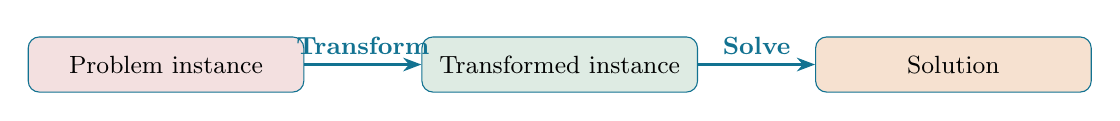
\begin{tikzpicture}[
    box/.style={draw=PrimaryMid,fill=PrimaryLight!30,rounded corners=4pt,
                font=\small,minimum width=3.5cm,minimum height=0.7cm,text centered},
    arr/.style={-{Stealth},PrimaryMid,thick}
  ]
    \node[box,fill=AlertRed!15] (prob) at (0,0) {Problem instance};
    \node[box,fill=SuccessGreen!15] (trans) at (5.0,0) {Transformed instance};
    \node[box,fill=AccentOrange!20] (sol) at (10,0) {Solution};
    \draw[arr] (prob) -- node[above,font=\small]{\textbf{Transform}} (trans);
    \draw[arr] (trans) -- node[above,font=\small]{\textbf{Solve}} (sol);
  \end{tikzpicture}
  \vspace{0.5em}
  \begin{columns}[T]
    \column{0.32\textwidth}
      \begin{block}{1. Instance simplification}
        Transform to a simpler/easier instance of the \emph{same} problem.\\[0.3em]
        \emph{Example:} presort before searching
      \end{block}
    \column{0.32\textwidth}
      \begin{block}{2. Representation change}
        Transform to a different \emph{data structure} for the same instance.\\[0.3em]
        \emph{Example:} AVL tree, heap
      \end{block}
    \column{0.32\textwidth}
      \begin{block}{3. Problem reduction}
        Transform to a \emph{different} problem with a known algorithm.\\[0.3em]
        \emph{Example:} LCM via GCD
      \end{block}
  \end{columns}
\end{frame}

% ============================================================
\section{Instance Simplification — Presorting}
% ============================================================

\begin{frame}[shrink=20]{Presorting}
  \begin{block}{Idea}
    Many problems become \emph{much easier} on a sorted list.
    Sort once in $\Theta(n\log n)$, then exploit order repeatedly.
  \end{block}
  \vspace{0.3em}
  \begin{columns}[T]
    \column{0.50\textwidth}
      \textbf{Example 1: Element uniqueness}
      \begin{itemize}
        \item Brute force: compare all pairs → $\mathcal{O}(n^2)$
        \item Presort + scan adjacent pairs → $\Theta(n\log n)$
      \end{itemize}
      \begin{algorithmic}[1]
        \State sort $A$
        \For{$i \gets 0$ \textbf{to} $n-2$}
          \If{$A[i] = A[i+1]$} \Return \textbf{false} \EndIf
        \EndFor
        \State \Return \textbf{true}
      \end{algorithmic}

      \vspace{0.2em}
      \scriptsize
      \begin{tabular}{@{}lll@{}}
        \toprule
        \textbf{Problem} & \textbf{Brute force} & \textbf{After presort} \\
        \midrule
        Uniqueness & $\mathcal{O}(n^2)$ & $\Theta(n\log n)$ \\
        Mode       & $\mathcal{O}(n^2)$ & $\Theta(n\log n)$ \\
        Search/query & $\mathcal{O}(n)$ & $\mathcal{O}(\log n)$ \\
        \bottomrule
      \end{tabular}
    \column{0.46\textwidth}
      \textbf{Example 2: Mode (most frequent element)}
      \begin{itemize}
        \item Presort, then scan runs to find the longest
      \end{itemize}
      \vspace{0.3em}
      \textbf{Example 3: Searching with many queries}
      \begin{itemize}
        \item Presort once in $\Theta(n\log n)$
        \item Each binary search query: $\mathcal{O}(\log n)$
        \item Break-even vs. sequential: $\approx \log n$ queries
      \end{itemize}
      \vspace{0.4em}
      \begin{alertblock}{Key question}
        Is the $\Theta(n\log n)$ presorting cost worth paying?\\
        \textbf{Yes} if you execute \emph{many queries} on the same data.\\
        \textbf{No} if you only need one answer.
      \end{alertblock}
  \end{columns}
\end{frame}

% ============================================================
\section{Representation Change — Balanced Trees}
% ============================================================

\begin{frame}[shrink=12]{Binary Search Trees — The Problem}
  \begin{columns}[T]
    \column{0.50\textwidth}
      BST operations (search, insert, delete) depend on \emph{height}:
      \begin{itemize}
        \item Best (balanced): $h = \lfloor\log_2 n\rfloor$ → $\Theta(\log n)$
        \item Worst (sorted input): $h = n-1$ → $\Theta(n)$
      \end{itemize}
      \vspace{0.3em}
      \begin{alertblock}{The problem}
        Inserting sorted data into a BST produces a \emph{linear chain} —
        as slow as sequential search!
      \end{alertblock}
      \vspace{0.3em}
      \textbf{Solution:} Keep the tree \emph{balanced} after every
      insertion/deletion.
    \column{0.45\textwidth}
      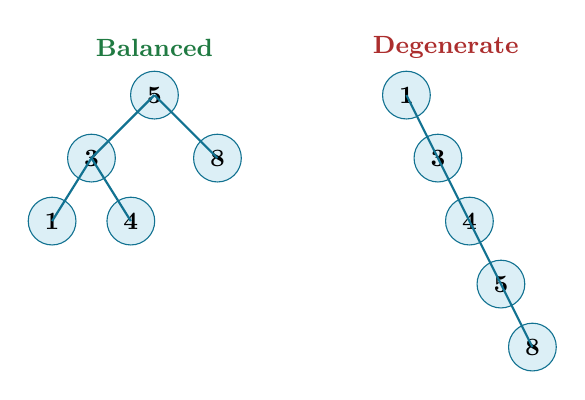
\begin{tikzpicture}[
        nd/.style={circle,draw=PrimaryMid,fill=PrimaryLight!50,
                   font=\bfseries\small,minimum size=0.6cm}
      ]
        \node[font=\small\bfseries,text=SuccessGreen] at (0.8,3.6) {Balanced};
        \node[nd] at (0.8,3.0) {5};
        \node[nd] at (0.0,2.2) {3};
        \node[nd] at (1.6,2.2) {8};
        \node[nd] at (-0.5,1.4) {1};
        \node[nd] at (0.5,1.4) {4};
        \draw[PrimaryMid,thick] (0.8,3.0)--(0,2.2)--(-0.5,1.4);
        \draw[PrimaryMid,thick] (0.8,3.0)--(1.6,2.2);
        \draw[PrimaryMid,thick] (0,2.2)--(0.5,1.4);

        \node[font=\small\bfseries,text=AlertRed] at (4.5,3.6) {Degenerate};
        \node[nd] at (4.0,3.0) {1};
        \node[nd] at (4.4,2.2) {3};
        \node[nd] at (4.8,1.4) {4};
        \node[nd] at (5.2,0.6) {5};
        \node[nd] at (5.6,-0.2){8};
        \draw[PrimaryMid,thick]
          (4.0,3.0)--(4.4,2.2)--(4.8,1.4)--(5.2,0.6)--(5.6,-0.2);
      \end{tikzpicture}
  \end{columns}
\end{frame}

\begin{frame}[shrink=12]{AVL Trees}
  \begin{block}{Definition}
    An \keyword{AVL tree} is a BST where for every node, the
    \emph{balance factor} (height of left subtree minus height of right
    subtree) is $-1$, $0$, or $+1$.
  \end{block}
  \vspace{0.3em}
  \begin{columns}[T]
    \column{0.50\textwidth}
      \textbf{Rebalancing rotations} (when a new node violates balance):
      \begin{itemize}
        \item \keyword{Single R-rotation}: left-left imbalance
        \item \keyword{Single L-rotation}: right-right imbalance
        \item \keyword{Double LR-rotation}: left-right imbalance
        \item \keyword{Double RL-rotation}: right-left imbalance
      \end{itemize}
      \vspace{0.3em}
      \textbf{Guaranteed height:}
      \[
        h \leq 1.44\log_2(n+2) - 1.33
      \]
      All operations: $\mathcal{O}(\log n)$ worst case.
    \column{0.45\textwidth}
      \textbf{Single R-rotation example:}
      \vspace{0.2em}
      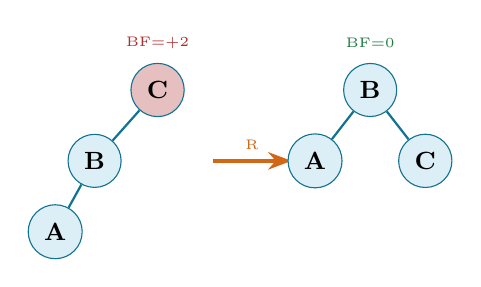
\begin{tikzpicture}[
        nd/.style={circle,draw=PrimaryMid,fill=PrimaryLight!50,
                   font=\bfseries\small,minimum size=0.55cm},
        arr/.style={-{Stealth},AccentOrange,very thick}
      ]
        % Before
        \node[nd,fill=AlertRed!30] (c) at (0.8,2.5) {C};
        \node[nd] (b) at (0.0,1.6) {B};
        \node[nd] (a) at (-0.5,0.7) {A};
        \draw[PrimaryMid,thick] (c)--(b)--(a);
        \node[font=\tiny,text=AlertRed] at (0.8,3.1) {BF=+2};
        % Arrow
        \draw[arr] (1.5,1.6) -- (2.5,1.6) node[midway,above,font=\tiny]{R};
        % After
        \node[nd] (b2) at (3.5,2.5) {B};
        \node[nd] (a2) at (2.8,1.6) {A};
        \node[nd] (c2) at (4.2,1.6) {C};
        \draw[PrimaryMid,thick] (b2)--(a2); \draw[PrimaryMid,thick] (b2)--(c2);
        \node[font=\tiny,text=SuccessGreen] at (3.5,3.1) {BF=0};
      \end{tikzpicture}
      \vspace{0.2em}
      \textbf{Construction: insert 5,6,8,3,2,4,7}\\
      (worked trace: 4 rotations needed)
  \end{columns}
\end{frame}

\begin{frame}[shrink=12]{2-3 Trees}
  \begin{columns}[T]
    \column{0.55\textwidth}
      \begin{block}{Definition}
        A \keyword{2-3 tree} is a balanced search tree where:
        \begin{itemize}
          \item Every node has 2 or 3 children (internal nodes)
          \item All leaves are at the \emph{same level}
        \end{itemize}
      \end{block}
      \vspace{0.3em}
      \textbf{Insertion:} insert at a leaf; if a 3-node overflows,
      \emph{split} it and push the middle key up.

      \vspace{0.3em}
      \textbf{Height bounds:}
      \[
        \log_3(n+1)-1 \leq h \leq \log_2(n+1)-1
      \]
      All operations: $\Theta(\log n)$
    \column{0.40\textwidth}
      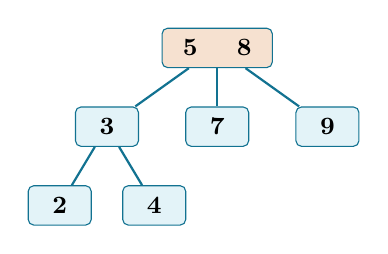
\begin{tikzpicture}[
        twonode/.style={draw=PrimaryMid,fill=PrimaryLight!40,rounded corners=2pt,
                        font=\small\bfseries,minimum width=0.8cm,
                        minimum height=0.5cm,text centered},
        threenode/.style={draw=PrimaryMid,fill=AccentOrange!20,rounded corners=2pt,
                          font=\small\bfseries,minimum width=1.4cm,
                          minimum height=0.5cm,text centered},
        arr/.style={draw=PrimaryMid,thick}
      ]
        \node[threenode] (r) at (2.0,3.0) {5 \quad 8};
        \node[twonode]   (l) at (0.6,2.0) {3};
        \node[twonode]   (m) at (2.0,2.0) {7};
        \node[twonode]   (ri) at (3.4,2.0){9};
        \node[twonode]   (ll) at (0.0,1.0) {2};
        \node[twonode]   (lr) at (1.2,1.0) {4};
        \draw[arr] (r)--(l); \draw[arr] (r)--(m); \draw[arr] (r)--(ri);
        \draw[arr] (l)--(ll); \draw[arr] (l)--(lr);
      \end{tikzpicture}
      \vspace{0.3em}
      \textbf{Generalisations:} 2-3-4 trees, B-trees (used in
      databases and file systems for disk-block efficiency)
  \end{columns}
\end{frame}

% ============================================================
\section{Representation Change — Heaps \& Heapsort}
% ============================================================

\begin{frame}[shrink=12]{Heaps}
  \begin{block}{Definition}
    A \keyword{heap} is a complete binary tree where every node's key
    is $\geq$ its children's keys (\emph{max-heap}).
  \end{block}
  \vspace{0.3em}
  \begin{columns}[T]
    \column{0.50\textwidth}
      \textbf{Key properties:}
      \begin{itemize}
        \item Height: $\lfloor\log_2 n\rfloor$ — always balanced
        \item Root holds the \emph{maximum} key
        \item Stored as an array (left-to-right, level by level):
          \begin{itemize}
            \item Left child of $j$: index $2j$
            \item Right child of $j$: index $2j+1$
            \item Parent of $j$: index $\lfloor j/2\rfloor$
          \end{itemize}
      \end{itemize}
    \column{0.45\textwidth}
      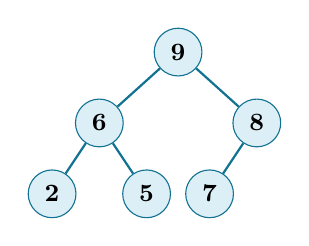
\begin{tikzpicture}[
        nd/.style={circle,draw=PrimaryMid,fill=PrimaryLight!50,
                   font=\bfseries\small,minimum size=0.6cm}
      ]
        \node[nd] (9) at (2.0,3.0) {9};
        \node[nd] (6) at (1.0,2.1) {6};
        \node[nd] (8) at (3.0,2.1) {8};
        \node[nd] (2) at (0.4,1.2) {2};
        \node[nd] (5) at (1.6,1.2) {5};
        \node[nd] (7) at (2.4,1.2) {7};
        \draw[PrimaryMid,thick]
          (9)--(6)--(2) (6)--(5) (9)--(8)--(7);
      \end{tikzpicture}

      \textbf{Array}: \quad
      \begin{tabular}{|c|c|c|c|c|c|}
        \hline
        \rowcolor{PrimaryLight!40}
        9 & 6 & 8 & 2 & 5 & 7 \\
        \hline
        1 & 2 & 3 & 4 & 5 & 6 \\
        \hline
      \end{tabular}
  \end{columns}
\end{frame}

\begin{frame}[shrink=12]{Heapsort}
  \begin{columns}[T]
    \column{0.50\textwidth}
      \textbf{Stage 1 — Build heap} (bottom-up):
      Start from last parental node; sift down each node.
      Complexity: $\Theta(n)$

      \vspace{0.3em}
      \textbf{Stage 2 — Sort} (repeated max deletion):
      \begin{enumerate}
        \item Swap root (max) with last element
        \item Shrink heap by 1
        \item Sift down new root
        \item Repeat $n-1$ times
      \end{enumerate}
      Complexity: $\Theta(n\log n)$

      \vspace{0.3em}
      \textbf{Total:} $\Theta(n) + \Theta(n\log n) = \Theta(n\log n)$
    \column{0.45\textwidth}
      \textbf{Sorting $[2,\,9,\,7,\,6,\,5,\,8]$:}
      \vspace{0.2em}

      \begin{tabular}{cccccc}
        \multicolumn{6}{l}{\scriptsize After build-heap:} \\
        \rowcolor{PrimaryLight!40}
        9&6&8&2&5&7 \\[2pt]
        \multicolumn{6}{l}{\scriptsize After extraction 1:} \\
        \rowcolor{white}
        7&6&8&2&5&\cellcolor{SuccessGreen!20}9 \\[2pt]
        \multicolumn{6}{l}{\scriptsize After sift-down:} \\
        \rowcolor{PrimaryLight!40}
        8&6&7&2&5&\cellcolor{SuccessGreen!20}9 \\[2pt]
        \multicolumn{6}{l}{\scriptsize \ldots continues \ldots} \\
        \rowcolor{SuccessGreen!20}
        2&5&6&7&8&9 \\
      \end{tabular}
      \vspace{0.3em}
      In-place: \textcolor{SuccessGreen}{Yes} \quad Stable: \alert{No}
  \end{columns}
\end{frame}

% ============================================================
\section{Problem Reduction}
% ============================================================

\begin{frame}[shrink=12]{Problem Reduction — Concept}
  \begin{block}{Idea}
    Solve problem A by transforming it into problem B for which
    an efficient algorithm is already known.
  \end{block}
  \vspace{0.3em}
  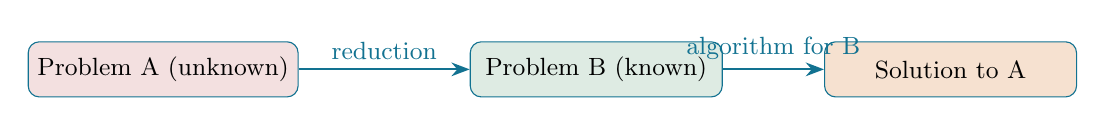
\begin{tikzpicture}[
    box/.style={draw=PrimaryMid,fill=PrimaryLight!30,rounded corners=4pt,
                font=\small,minimum width=3.2cm,minimum height=0.7cm,text centered},
    arr/.style={-{Stealth},PrimaryMid,thick}
  ]
    \node[box,fill=AlertRed!15] (A) at (0,0) {Problem A (unknown)};
    \node[box,fill=SuccessGreen!15] (B) at (5.5,0) {Problem B (known)};
    \node[box,fill=AccentOrange!20] (S) at (10,0) {Solution to A};
    \draw[arr] (A)--node[above,font=\small]{reduction}(B);
    \draw[arr] (B)--node[above,font=\small]{algorithm for B}(S);
  \end{tikzpicture}
  \vspace{0.4em}
  \begin{columns}[T]
    \column{0.48\textwidth}
      \textbf{Classic examples:}
      \begin{itemize}
        \item $\mathrm{lcm}(m,n) = mn/\gcd(m,n)$ — reduce LCM to GCD
        \item Paths of length $k$ in graph: compute $A^k$ (matrix power)
        \item Minimisation $\to$ maximisation: negate objective
      \end{itemize}
    \column{0.48\textwidth}
      \begin{alertblock}{Requirement for usefulness}
        The combined cost of the reduction \emph{plus} solving B must
        be less than the best direct algorithm for A.
      \end{alertblock}
  \end{columns}
\end{frame}

\begin{frame}[shrink=28]{LCM via GCD}
  \begin{columns}[T]
    \column{0.50\textwidth}
      \begin{block}{Theorem}
        For any positive integers $m, n$:
        \[
          \mathrm{lcm}(m,n) = \frac{m \cdot n}{\gcd(m,n)}
        \]
      \end{block}
      \vspace{0.3em}
      \textbf{Algorithm:}
      \begin{enumerate}
        \item Compute $\gcd(m,n)$ using Euclid's algorithm — $\mathcal{O}(\log n)$
        \item Return $m \,/\, \gcd(m,n) \cdot n$ — $\mathcal{O}(1)$
      \end{enumerate}
      \vspace{0.3em}
      \textbf{Example:} $\mathrm{lcm}(24,\,60)$
      \begin{itemize}
        \item $\gcd(24,60) = 12$
        \item $\mathrm{lcm}(24,60) = 24 \times 60 / 12 = \highlight{120}$
      \end{itemize}

    \column{0.46\textwidth}
      % Reduction flow diagram
      \begin{center}
      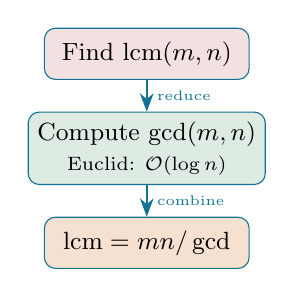
\begin{tikzpicture}[
        rbox/.style={draw=PrimaryMid,fill=PrimaryLight!30,rounded corners=4pt,
                     font=\small,minimum width=2.6cm,minimum height=0.65cm,
                     align=center},
        arr/.style={-{Stealth},PrimaryMid,thick}
      ]
        \node[rbox,fill=AlertRed!15]      (lcm) at (0,2.0)  {Find $\mathrm{lcm}(m,n)$};
        \node[rbox,fill=SuccessGreen!15]  (gcd) at (0,0.8)  {Compute $\gcd(m,n)$\\{\scriptsize Euclid: $\mathcal{O}(\log n)$}};
        \node[rbox,fill=AccentOrange!20]  (sol) at (0,-0.4) {$\mathrm{lcm} = mn/\gcd$};
        \draw[arr] (lcm) -- node[right,font=\tiny]{reduce} (gcd);
        \draw[arr] (gcd) -- node[right,font=\tiny]{combine} (sol);
      \end{tikzpicture}
      \end{center}
      \vspace{0.2em}
      \textbf{Alternative (brute force):} $24 = 2^3\!\cdot 3$,\;
      $60 = 2^2\!\cdot 3\cdot 5$
      \[
        \mathrm{lcm} = 2^3 \cdot 3 \cdot 5 = 120
      \]
      Requires prime factorisation — much slower.
      \begin{exampleblock}{Lesson}
        Reduction to GCD turns an apparently hard problem (LCM)
        into a one-liner with $\mathcal{O}(\log n)$ complexity.
      \end{exampleblock}
  \end{columns}
\end{frame}

% ============================================================
\section{Linear Programming}
% ============================================================

\begin{frame}[shrink=12]{Linear Programming — Introduction}
  \begin{block}{Definition}
    A \keyword{Linear Program (LP)} maximises (or minimises) a
    \emph{linear} objective function subject to \emph{linear}
    inequality/equality constraints.
  \end{block}

  \[
    \text{maximise/minimise}\quad c_1x_1 + \cdots + c_nx_n
    \quad\text{subject to}\quad
    a_{i1}x_1 + \cdots + a_{in}x_n \;\leq/\geq/=\; b_i,\;
    x_j \geq 0
  \]
 
  \begin{columns}[T]
    \column{0.48\textwidth}
      \textbf{Components:}
      \begin{itemize}
        \item \concept{Decision variables}: $x_1,\ldots,x_n$
        \item \concept{Objective function}: linear in $x_j$
        \item \concept{Constraints}: linear inequalities/equalities
        \item \concept{Non-negativity}: $x_j \geq 0$
      \end{itemize}
    \column{0.48\textwidth}
      \textbf{Properties:}
      \begin{itemize}
        \item \emph{Feasible region}: convex polygon/polyhedron
        \item \emph{Optimal solution}: always at a vertex
        \item Solvable in polynomial time (ellipsoid method,
              interior-point methods)
        \item Simplex: efficient in practice
      \end{itemize}
  \end{columns}
\end{frame}

\begin{frame}[shrink=12]{LP Example: Production Planning}
  \begin{columns}[T]
    \column{0.55\textwidth}
      \textbf{Problem:} A factory produces chocolates A and B.
      Resources (per unit): A needs 1 Milk + 3 Choco; B needs 1 Milk + 2 Choco.
      Available: 5 Milk, 12 Choco. Profit: 6 SAR/unit A, 5 SAR/unit B.
      Maximise profit.

      \vspace{0.3em}
      \textbf{LP formulation:}
      \begin{alignat}{2}
        \text{max}\quad & 6X + 5Y \\
        \text{s.t.}\quad & X + Y \leq 5 \\
                         & 3X + 2Y \leq 12 \\
                         & X, Y \geq 0
      \end{alignat}
    \column{0.40\textwidth}
      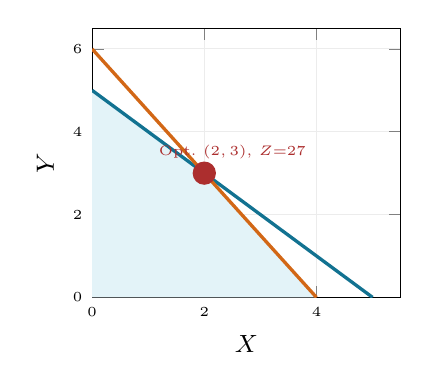
\begin{tikzpicture}
        \begin{axis}[
          width=5.5cm,height=5.0cm,
          xlabel={$X$},ylabel={$Y$},
          xmin=0,xmax=5.5,ymin=0,ymax=6.5,
          tick label style={font=\tiny},
          label style={font=\small},
          grid=major,grid style={gray!15}
        ]
          % Feasible region (filled)
          \addplot[fill=PrimaryLight!40,draw=none] coordinates
            {(0,0)(0,5)(2,3)(4,0)} -- cycle;
          \addplot[PrimaryMid,very thick] coordinates {(0,5)(5,0)};
          \addplot[AccentOrange,very thick] coordinates {(0,6)(4,0)};
          % Optimal point
          \addplot[mark=*,AlertRed,mark size=4pt] coordinates {(2,3)};
          \node[font=\tiny,text=AlertRed] at (axis cs:2.5,3.5)
            {Opt.\ $(2,3)$, $Z{=}27$};
        \end{axis}
      \end{tikzpicture}
  \end{columns}
\end{frame}

\begin{frame}[shrink=12]{Reducing the 0-1 Knapsack to an LP}
  \begin{columns}[T]
    \column{0.55\textwidth}
      \textbf{0-1 Knapsack} as an Integer Linear Program (ILP):
      \[
        \text{max}\;\sum_{j=1}^n v_j x_j
        \quad\text{s.t.}\;\sum_{j=1}^n w_j x_j \leq W,\;
        x_j \in \{0,1\}
      \]
      \vspace{0.3em}
      \textbf{Example ($W=10$):}
      \begin{tabular}{lrrr}
        \toprule
        & $w$ & $v$ & $x^*$ \\
        \midrule
        Item 1 & 7 & 42 & 0 \\
        Item 2 & 3 & 12 & 0 \\
        Item 3 & 4 & 40 & \textcolor{SuccessGreen}{1} \\
        Item 4 & 5 & 25 & \textcolor{SuccessGreen}{1} \\
        \bottomrule
      \end{tabular}
      \vspace{0.2em}
      Optimal: items 3+4, value = \highlight{65}, weight = 9
    \column{0.40\textwidth}
      \begin{alertblock}{ILP is harder than LP}
        Adding integrality constraints makes the problem NP-hard.
        Solving it exactly requires branch-and-bound or
        dynamic programming.
      \end{alertblock}
      \vspace{0.3em}
      \begin{exampleblock}{LP relaxation}
        Remove $x_j\in\{0,1\}$; allow $0\leq x_j\leq 1$.
        This gives an upper bound and is solvable in polynomial time.
        Rounding the LP solution gives a heuristic.
      \end{exampleblock}
  \end{columns}
\end{frame}

% ── Chapter Summary ──────────────────────────────────────────
\begin{frame}[shrink=12]{Chapter 5 Summary}
  \begin{columns}[T]
    \column{0.55\textwidth}
      \textbf{Three flavours of Transform \& Conquer:}
      \begin{enumerate}
        \item \keyword{Presorting} — $\Theta(n\log n)$ once, then fast queries
        \item \keyword{Representation change}
          \begin{itemize}
            \item AVL trees: $\mathcal{O}(\log n)$ all ops
            \item 2-3 trees: $\Theta(\log n)$ all ops
            \item Heaps: $\mathcal{O}(\log n)$ insert/delete-max
            \item Heapsort: $\Theta(n\log n)$, in-place
          \end{itemize}
        \item \keyword{Problem reduction}
          \begin{itemize}
            \item LCM $\to$ GCD, graph paths $\to$ matrix power
            \item LP as a reduction target for optimisation
          \end{itemize}
      \end{enumerate}
    \column{0.40\textwidth}
      \begin{block}{Next chapter}
        \textbf{Chapter 6:} Dynamic Programming — solving problems
        with \emph{overlapping sub-problems} by filling a table
        bottom-up (or top-down with memoisation).
      \end{block}
      \vspace{0.3em}
      \begin{exampleblock}{Self-check}
        \begin{enumerate}
          \item When is presorting beneficial?
          \item What rotation fixes a left-right imbalance in an AVL tree?
          \item What is the difference between LP and ILP?
        \end{enumerate}
      \end{exampleblock}
  \end{columns}
\end{frame}

\end{document}
